\subsection{Air Thermoregulation}
\label{sec:airthermoregulation}

\textbf{Purpose}: Maintaining desired leaf-zone air temperature and circulating air.

\textbf{Function}:
\begin{itemize}
    \item \textbf{Inputs}: Power, air temperature control signal (\ref{sec:automation}), air circulation control signal (\ref{sec:automation});
    \item \textbf{Outputs}: $\pm$Heat to environment, $\mp$heat to surroundings, internal air circulation, internal air temperature sensor signal (\ref{sec:automation});
\end{itemize}

\textbf{Method}:
\begin{enumerate}
    \item \textit{Testing}:
    \begin{itemize}
        \item Heat pump direction and magnitude respond to control signal as expected;
        \item Fans operate as expected;
        \item Heat pump power exceeds maximum heat loss (temperature extremes)\footnote{i.e. if X Watts leave the system at MAX$\degree$C internal, and Y Watts enter the system at MIN$\degree$C internal, the heat pump must transfer >X, >Y Watts.};
        \item Heat pump power exceeds that required to reach temperature extremes in under 120 seconds given the system's heat capacity;
    \end{itemize}
    \item \textit{Process}:
    \begin{enumerate}
        \item Air is circulated throughout the environment;
        \item Temperature is measured, sent to control module;
        \item Control module controls heat pump speed and direction (heating vs. cooling);
    \end{enumerate}
\end{enumerate}

\textbf{Calculations}:

Assuming an atmospheric pressure $P$ of 101.325kPa, a surroundings temperature range $T_{surr}$ of 22$\degree$C, a system target temperature range $T_{sys-min}$, $T_{sys-max}$ of 10-35$\degree$C, a molar mass of dry air\footnote{Water vapour has a maximum concentration of 30g/kg at 30$\degree$C, or 3\%, which is negligible for mass and heat capacity calculations.} $M$ of 28.97 $\frac g{mol}$, a specific heat capacity of dry air $c_p$ of $1.006 \frac{J}{g*\text{K}}$, a 4-unit (2x2 units, 16 faces) expanded configuration, and a face insulation RSI per mm of $0.0328\text{m}^2~  \degree \text{C}~\text{W}^{-1}~\text{mm}^{-1}$ (See Section \ref{sec:housing}):\\
\vspace{.05cm}
\begin{gather*}
    \label{eqn:heatloss}
    Q_{loss}=\frac{(T_{surr}-T_{sys-max}) * A}{\text{RSI per mm} * \ell}=\frac{(22\degree \text{C}-35\degree \text{C}) * (16 \text{ faces} * 0.5\text{m} * 0.5\text{m})}{0.0328 \text{m}^2~  \degree \text{C}~\text{W}^{-1}~\text{mm}^{-1} * 25.4 \text{mm}}=-62.42 W\\\vspace{.05cm}\\
    \label{eqn:heatgain}
    Q_{gain}=\frac{(T_{surr}-T_{sys-min}) * A}{\text{RSI per mm} * \ell}=\frac{(22\degree \text{C}-10\degree \text{C}) * (16 \text{ faces} * 0.5\text{m} * 0.5\text{m})}{0.0328 \text{m}^2~  \degree \text{C}~\text{W}^{-1}~\text{mm}^{-1} * 25.4 \text{mm}}=57.61 W\\\vspace{.05cm}\\
    \label{eqn:airmass}
    m_{air}=\frac{P*V*M}{R*T_{avg}}=\frac{101325\text{Pa}*(0.5\text{m}*0.5\text{m}*0.5\text{m}*4\text{ units})*28.97\frac g{mol}}{8.314\frac{J}{\text{mol}*K}*300\text{K}}=588.4g\\
    \vspace{1.5cm}\\
    \text{Continued on next page}
\end{gather*}
\vspace{1cm}

\begin{gather*}
  \label{eqn:heating}
  W_{heating}=\frac{m*c_p*(T_{surr}-T_{sys-max})}{t}=\frac{588.4g*1.006\frac{J}{g*\text{K}}*(22\degree \text{C}-35\degree \text{C})}{120\text{ sec}}=-64.13\text{W}\\
  \label{eqn:cooling}
  W_{cooling}=\frac{m*c_p*(T_{surr}-T_{sys-min})}{t}=\frac{588.4g*1.006\frac{J}{g*\text{K}}*(22\degree \text{C}-10\degree \text{C})}{120\text{ sec}}=59.19\text{W}
\end{gather*}

$\therefore$ A thermoelectric system able to transfer at least 70W (such as \cite{peltier}, which transfers up to 85W) will supply enough power to heat/cool the system from ambient to extremes in 120 seconds and maintain temperature.

\begin{gather*}
  \label{eqn:thermalresistance-hot}
  R_{\theta~Peltier-Surr}=R_{\theta~Peltier-Sink}+R_{\theta~Sink-Air}\le\frac{T_{h~max} - T_{surr}}{Q_{max}}=\frac{50\degree C - 22\degree C}{85W}=0.329\degree \text{C W}^{-1}\\
  \label{eqn:thermalresistance-cold}
  R_{\theta~Peltier-Sys}=R_{\theta~Peltier-Sink}+R_{\theta~Sink-Air}
\end{gather*}

\textbf{Features}:
\begin{itemize}
    \item \textit{Circulation Fans}: Located in growth environment to circulate air even temperature distribution.
    \item \textit{Temperature Sensors}: SHT31 \cite{sht31} sensors on breakout boards located throughout the growth environment to measure air temperature. Informs a \textbf{PID control loop} (\ref{sec:automation}).
    \item \textit{Heat Pump}: Pumps heat in or out of the growth environment. Is comprised of:
    \begin{itemize}
        \item \textit{Peltier Device}: 85W bidirectional solid-state \textbf{thermoelectric device} (aka Peltier tile) \cite{peltier} pumps heat from one face to the other. Better space efficiency, less complexity (no liquids, pressurized fluids, etc.), and more precise than other methods.
        \item \textit{Peltier Driver Circuit}: Controls magnitude and direction of Peltier device heat pump via a \textbf{dimmable voltage source} and \textbf{MOSFET H-bridge}, respectively. See Figure \ref{fig:peltierdriver}.
        \item \textit{Heat Sinks}: Aluminum blocks with fins hold and exchange heat between air and Peltier devices. One set on each side of the Peltier (inside and outside environment) builds "heat pump". Mating face coated with thermal compound for better transfer.
        \item \textit{Heat Sink Fans}: Located on both sets of heat sinks for better heat dissipation.
    \end{itemize}
\end{itemize}

\begin{figure}[h]
  \centering
  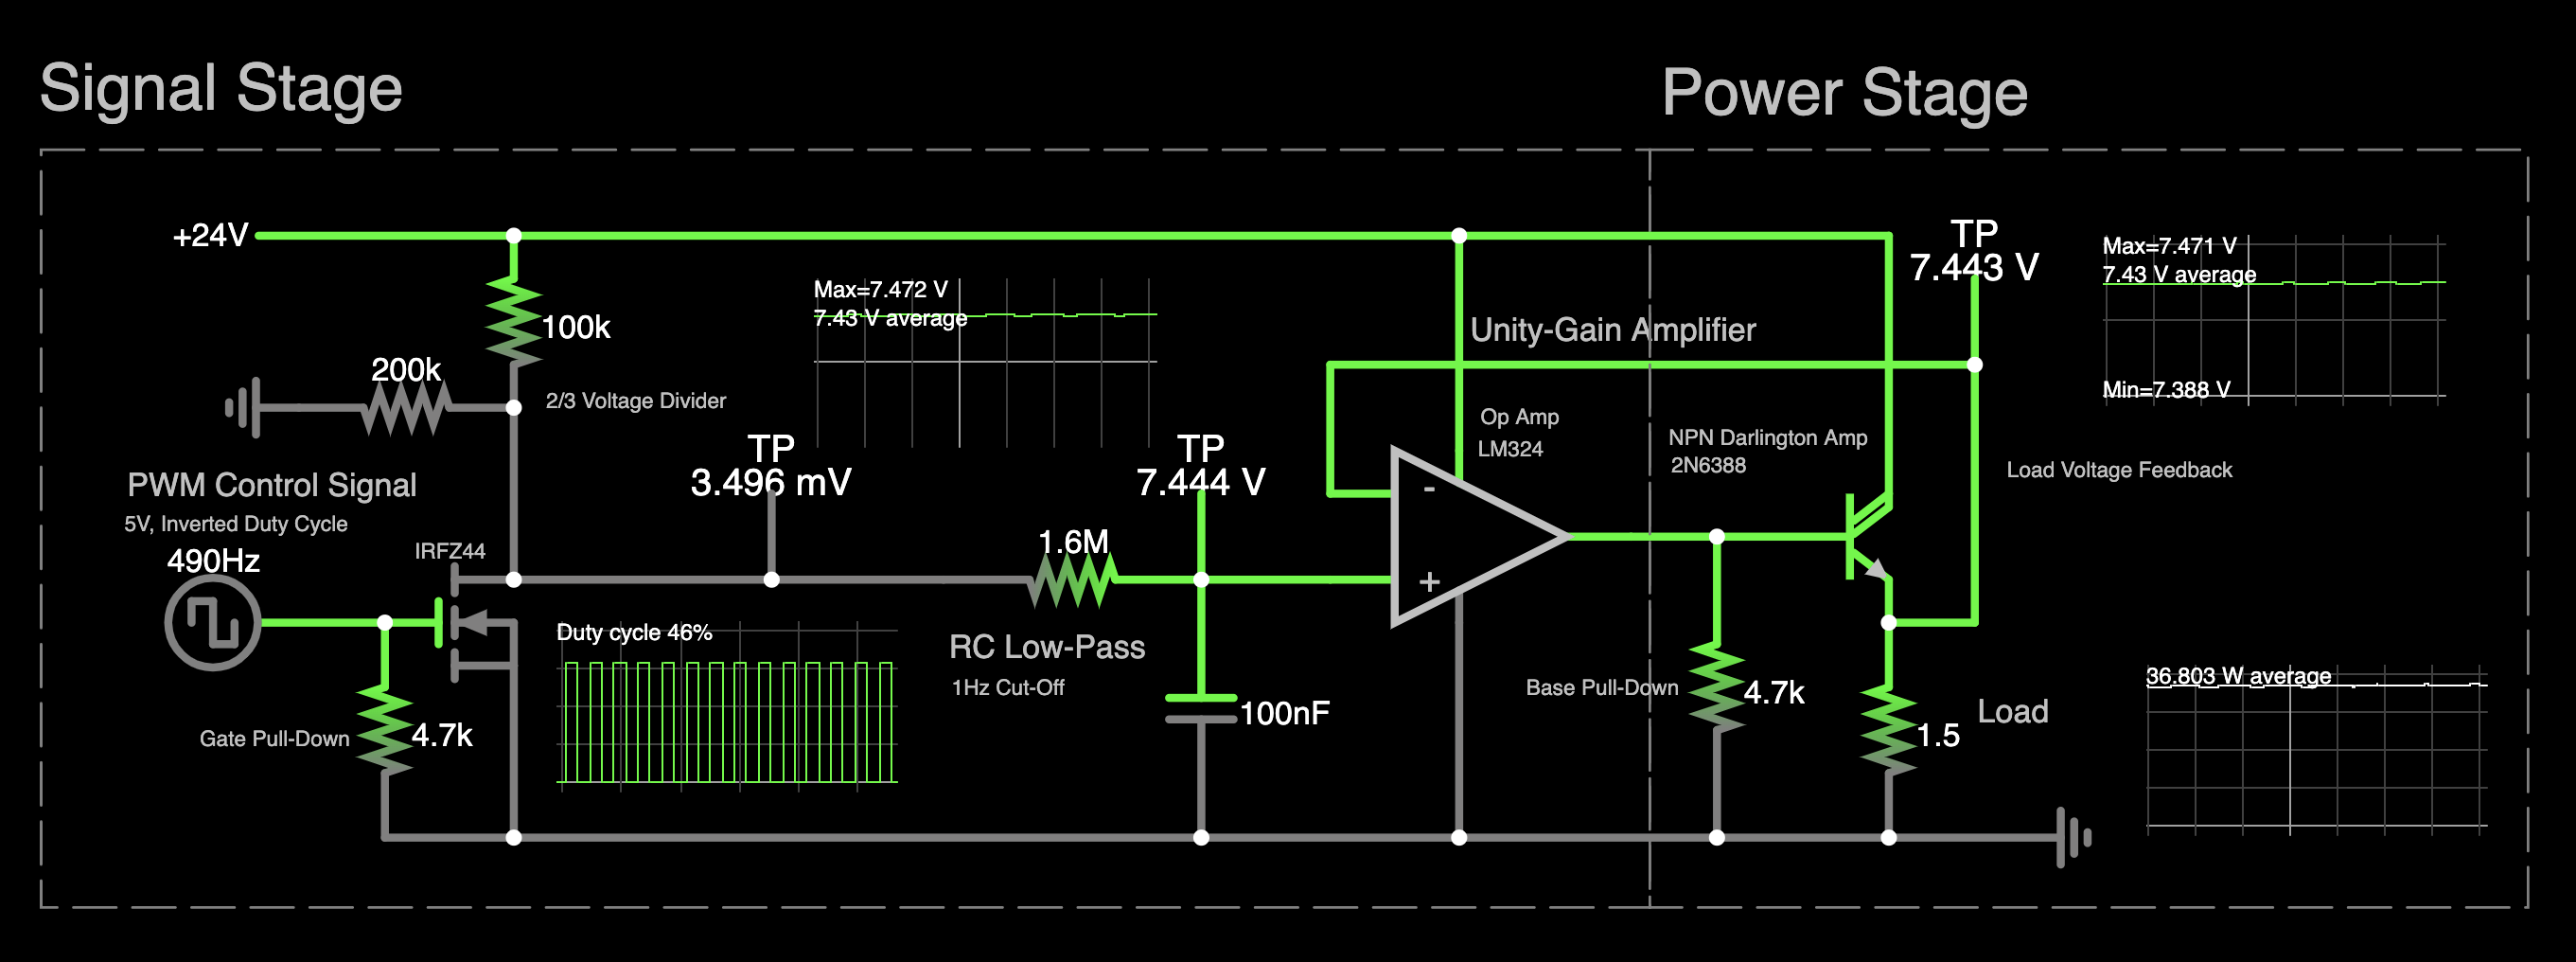
\includegraphics[width=0.8\textwidth]{images/thermosim.png}
  \hfill
  \caption{Peltier driver circuit simulation (live version: \cite{thermo-falstad})}
  \label{fig:peltierdriver}
\end{figure}